\title{\thesistitle} 
\author{\thesisauthor} 
\date{\thedate} 

\begin{titlepage}

\newgeometry{left=11mm,right=11mm,top=50mm,bottom=0pt}
\pagecolor{frontbackcolor}
\color{\frontpagetextcolour}

%{ % Thesis title (to change see Setup/Settings.tex) 
\Large
%\begin{tabular}{p{\linewidth}}
%\begin{tabular}{p{12000pt}}
\TitleFont{\thesistitle}\\
\large\thesissubtitle \\
\thesisauthor
%\end{tabular}
%}

% DTU department (to change see Setup/Settings.tex) 
\begin{tikzpicture}[remember picture,overlay]
\node[anchor=north east, 
      xshift=-10mm, 
      yshift=-12mm] 
      at (current page.north east) 
      {
        \color{\frontpagetextcolour}
        \begin{tabular}{r} 
        \textbf{\department} \\ 
        \departmentdescriber
        \end{tabular}
      }; 
\end{tikzpicture}

% DTU logo
\begin{tikzpicture}[remember picture,overlay]
\node[anchor=north west, 
      xshift=8.9mm, 
      yshift=-8.3mm] 
     at (current page.north west) 
     {\includegraphics[width=14.75mm,keepaspectratio]{Overleaf/Pictures/Logos/\dtulogocolour_\targetcolourmodel.pdf}}; 
\end{tikzpicture}

% Cover photo
\begin{tikzpicture}[remember picture,overlay]
\node[anchor=south, % anchor is bottom of picture
      xshift=0pt, 
      yshift=100mm] % shifting picture to actually be at the bottom of the page
     at (current page.south) % placement at bottom of the page
     {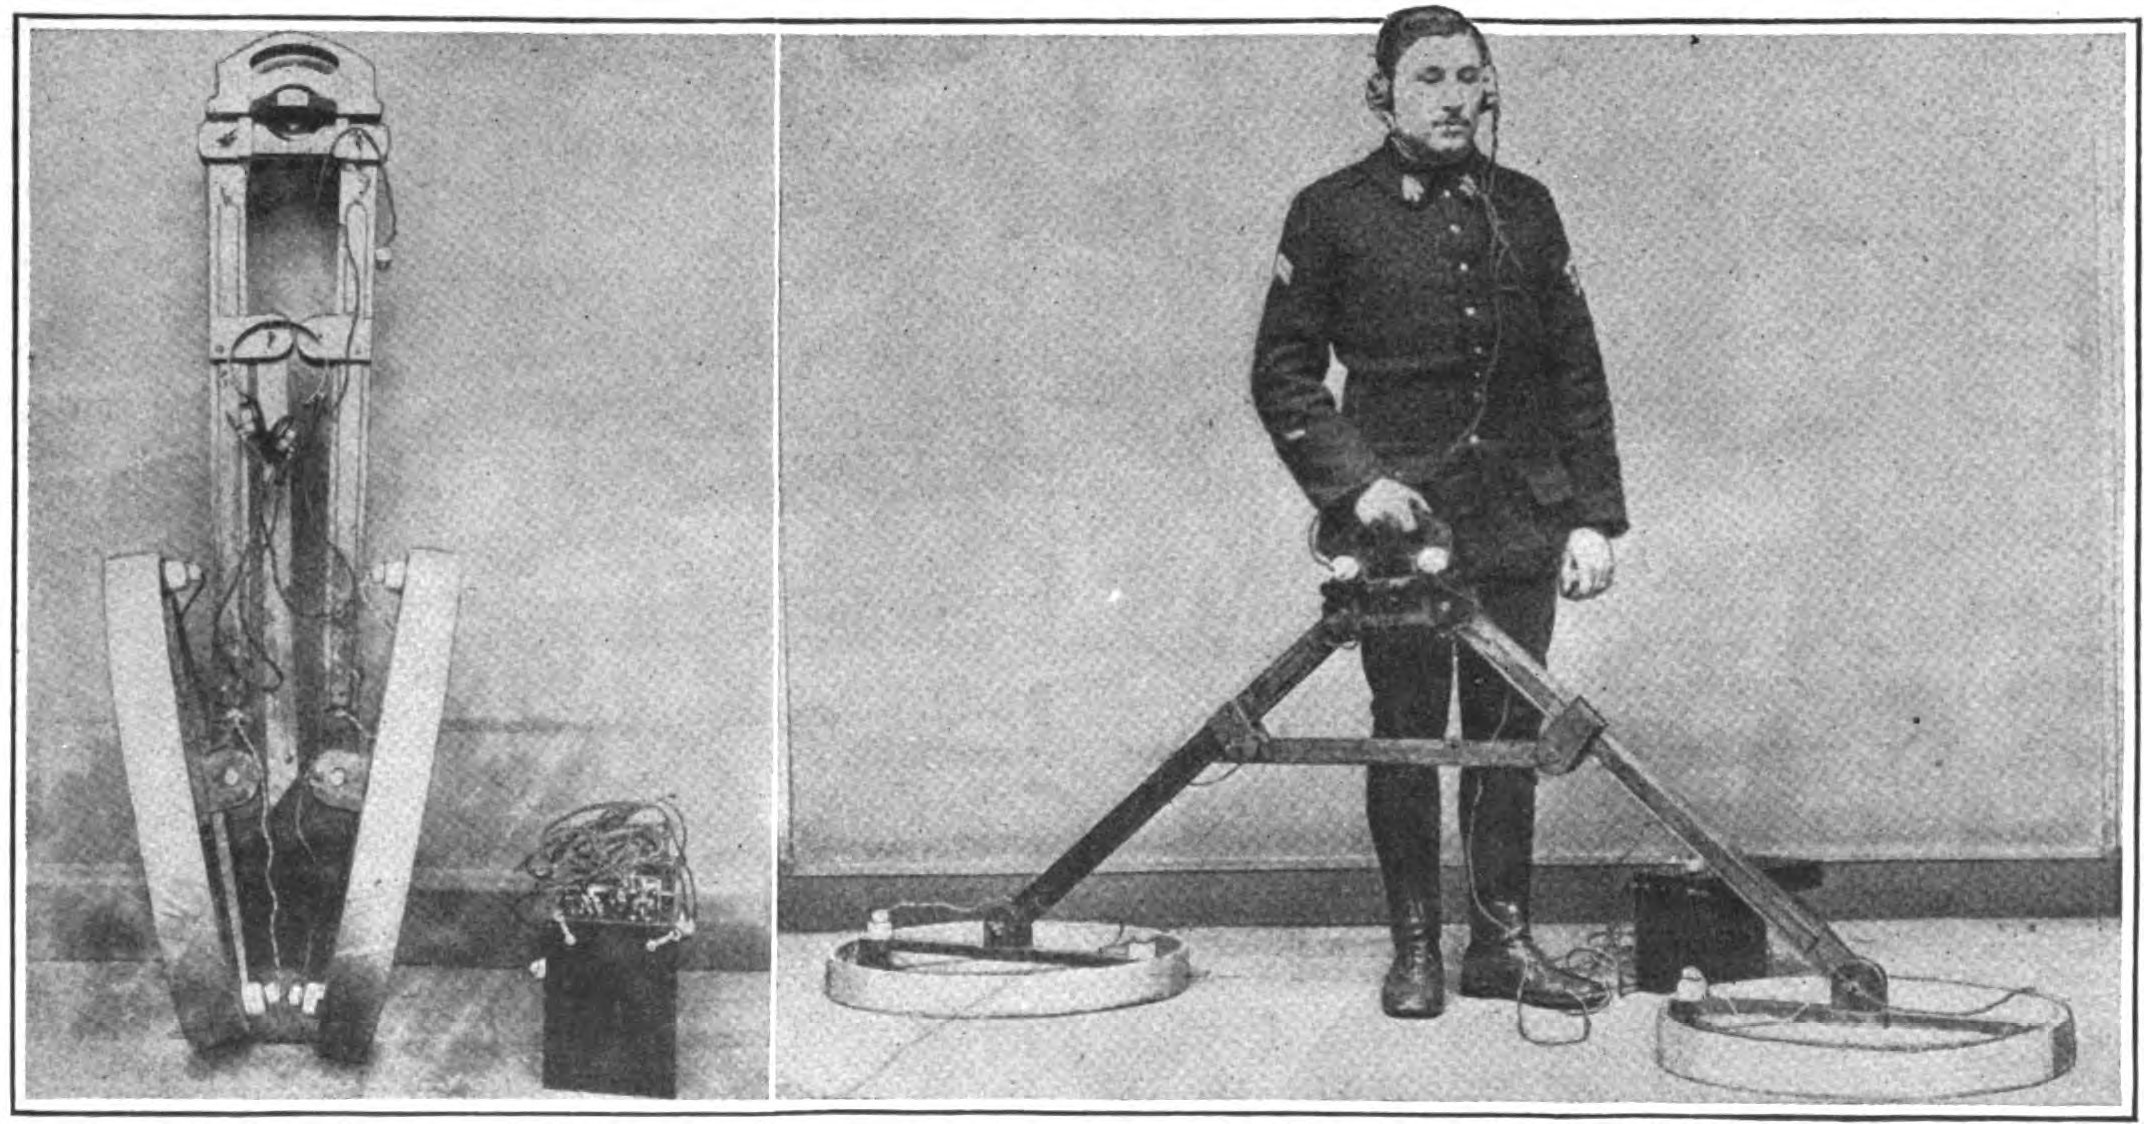
\includegraphics[width=21cm,keepaspectratio]{Overleaf/Pictures/Frontpage/Metal_detector_from_World_War_1.jpeg}};
\end{tikzpicture}

% Cover photo of us
\begin{figure}[b!]
    \captionsetup[subfigure]{font={sc,color=white}, labelformat=empty}
    \centering
    \vspace{1mm}
    \begin{subfigure}[1]{0.20\linewidth}
    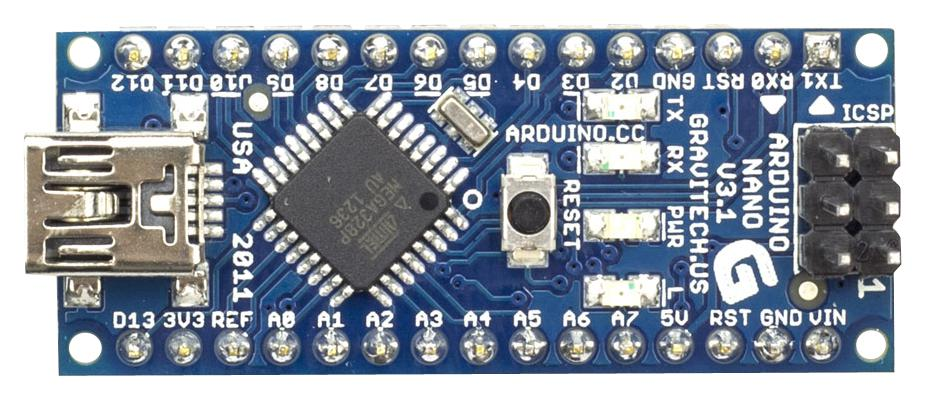
\includegraphics[width=\linewidth]{Overleaf/Pictures/Frontpage/ardrinon nano.jpg}
    \captionsetup{justification=centering}
    \caption[]{{\small xxxnavnxxx}\\{insæt std}}
    \end{subfigure}
    \hspace{2em}
    \begin{subfigure}[1]{0.20\linewidth}
    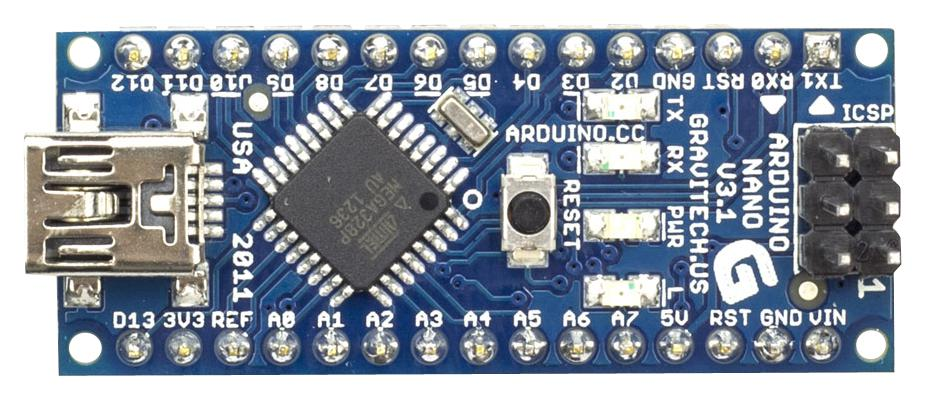
\includegraphics[width=\linewidth]{Overleaf/Pictures/Frontpage/ardrinon nano.jpg}
    \captionsetup{justification=centering}
    \caption[]{{\small xxxnavnxxx}\\{insæt std}}
    \end{subfigure}
    \hspace{2em}
    \begin{subfigure}[1]{0.20\linewidth}
    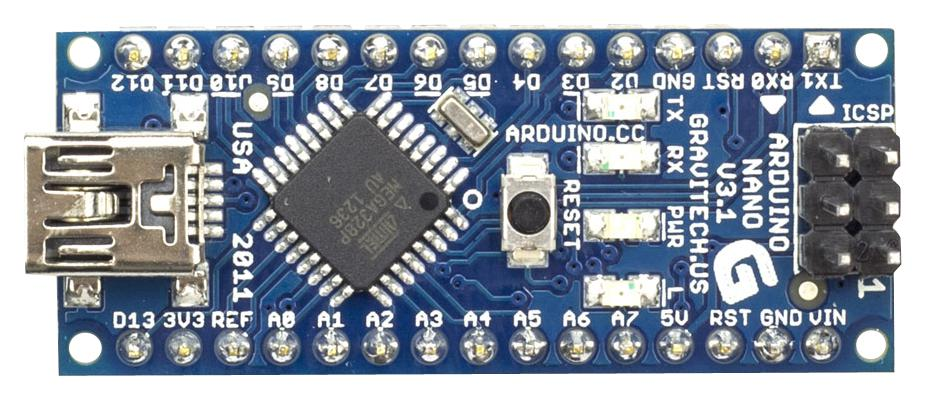
\includegraphics[width=\linewidth]{Overleaf/Pictures/Frontpage/ardrinon nano.jpg}
    \captionsetup{justification=centering}
    \caption[]{{\small xxxnavnxxx}\\{insæt std}}
    \end{subfigure}
    \hspace{2em}
    \vspace{20mm}
\end{figure}
\end{titlepage}